\documentclass[a4paper,12pt]{report}

\usepackage[english]{babel}
\usepackage[utf8]{inputenc}
\usepackage{indentfirst,setspace,subcaption}
\usepackage{amsmath,amssymb,graphicx,xcolor,url}
\usepackage{fancyhdr,tocbasic,titlesec,minted,listings}
\usepackage[a4paper,margin=24mm]{geometry}
\usepackage[skip=10pt plus1pt, indent=20pt]{parskip}
\usepackage[colorlinks=true,allcolors=blue,urlcolor=magenta]{hyperref}

\renewcommand{\thesection}{\arabic{section}}

% Header and footer styling
\pagestyle{fancy}
\setlength{\headheight}{15pt}
\fancyhf{}
\fancyhead[R]{\nouppercase\rightmark\hfill~Lab report}
\fancyfoot[C]{\hfill\thepage\hfill}

% TOC styling
\DeclareTOCStyleEntry[
  indent=12pt,
  level=1
]{largetocline}{section}

% Title page data
\title{Implementing Stack and Queue from scratch}
\author{Ngo Nguyen The Khoa -- 23127065 -- 23CLC09}
\date{June 3, 2024} % {\today}

\begin{document}

% Title page and TOC
\thispagestyle{empty}
\begin{titlepage}
	\begin{center}
		\makeatletter
		\newcommand{\HRule}{\rule{\linewidth}{0.4mm}}

		\textsc{\LARGE Vietnam National University,\\Ho Chi Minh City}\\[1.5cm]
		\textsc{\Large University of Science}\\[0.5cm]
		\textsc{\Large Faculty of Information Technology}\\[1.5cm]

		{\HRule}\\[1cm]
		{\huge \bfseries \@title}\\[0.5cm]
		{\HRule}\\[2cm]

		\textsc{\large CSC10004 -- Data Structures and Algorithms}\\[0.5cm]

		\vfill\vfill\vfill

		{\large \@author}\\[1.5cm]
		{\large \@date}
		\makeatother
	\end{center}
\end{titlepage}
\tableofcontents\thispagestyle{empty}

\pagebreak
\section{Result Screenshots}
\thispagestyle{empty}
\subsection{Stack (Array version)}
\subsubsection*{`push' operation}
\begin{figure}[!ht]
	\centering
	\begin{subfigure}{0.41\textwidth}
		\centering
		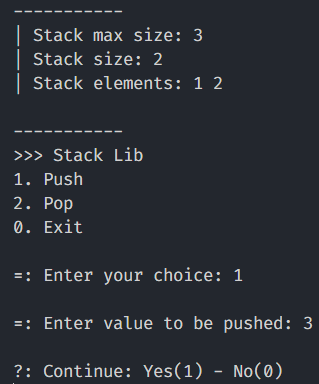
\includegraphics[width=\textwidth]{imgs/StackArray/push/normal.png}
		\caption{Normal test cases}\label{fig:stack_arr_push_normal}
	\end{subfigure}
	\hfill
	\begin{subfigure}{0.54\textwidth}
		\centering
		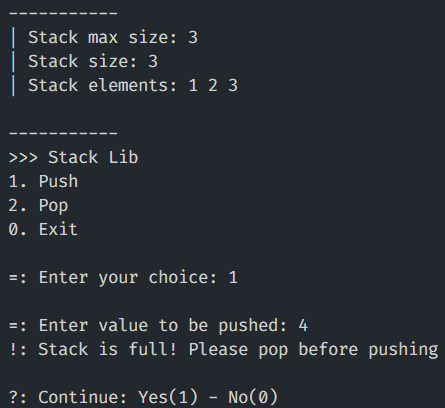
\includegraphics[width=\textwidth]{imgs/StackArray/push/full.png}
		\caption{When the stack is full}\label{fig:stack_arr_push_full}
	\end{subfigure}
	\hfill
	\begin{subfigure}{0.75\textwidth}
		\centering
		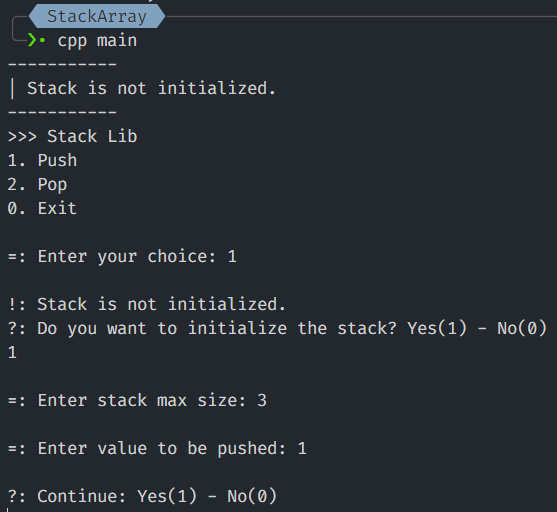
\includegraphics[width=\textwidth]{imgs/StackArray/push/empty.png}
		\caption{When the stack is uninitialized}\label{fig:stack_arr_push_empty}
	\end{subfigure}
	\caption{Screenshots of Stack (Array version) `push' operation.}\label{fig:stack_arr_push_cases}
\end{figure}
\subsubsection*{`pop' operation}
\begin{figure}[!ht]
	\centering
	\begin{subfigure}{0.58\textwidth}
		\centering
		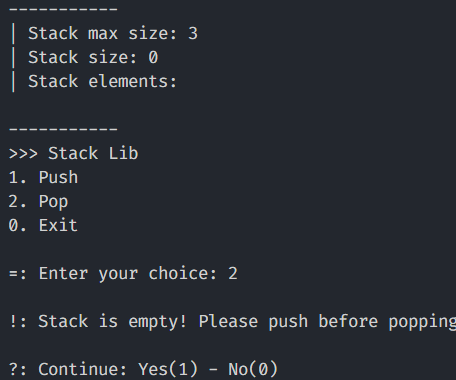
\includegraphics[width=\textwidth]{imgs/StackArray/pop/empty.png}
		\caption{When the stack is empty}\label{fig:stack_arr_pop_empty}
	\end{subfigure}
	\hfill
	\begin{subfigure}{0.39\textwidth}
		\centering
		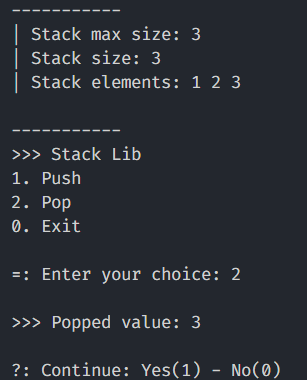
\includegraphics[width=\textwidth]{imgs/StackArray/pop/normal.png}
		\caption{Normal test cases}\label{fig:stack_arr_pop_normal}
	\end{subfigure}
	\caption{Screenshots of Stack (Array version) `pop' operation.}\label{fig:stack_arr_pop_cases}
\end{figure}

\pagebreak
\subsection{Stack (Linked List version)}
\subsubsection*{`push' operation}
\begin{figure}[!ht]
	\centering
	\begin{subfigure}{0.55\textwidth}
		\centering
		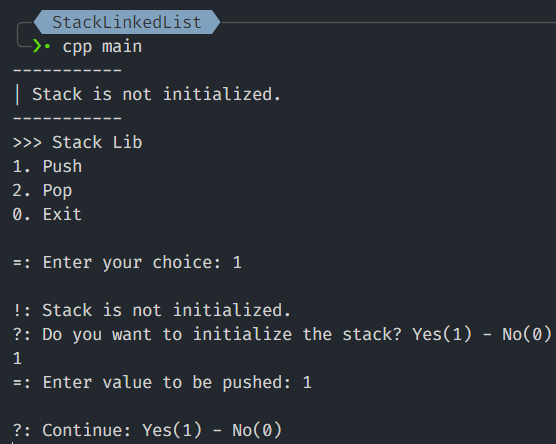
\includegraphics[width=\textwidth]{imgs/StackLinkedList/push/empty.png}
		\caption{When the stack is uninitialized}\label{fig:stack_ll_push_empty}
	\end{subfigure}
	\hfill
	\begin{subfigure}{0.43\textwidth}
		\centering
		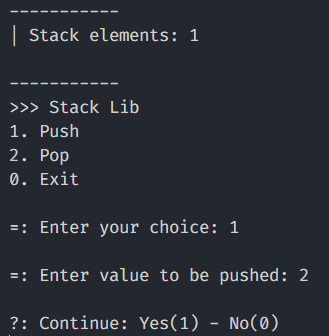
\includegraphics[width=\textwidth]{imgs/StackLinkedList/push/normal.png}
		\caption{Normal test cases}\label{fig:stack_ll_push_normal}
	\end{subfigure}
	\caption{Screenshots of Stack (Linked List version) `push' operation.}\label{fig:stack_ll_push_cases}
\end{figure}
\subsubsection*{`pop' operation}
\begin{figure}[!ht]
	\centering
	\begin{subfigure}{0.59\textwidth}
		\centering
		\includegraphics[width=\textwidth]{imgs/StackLinkedList/pop/empty.png}
		\caption{When the stack is empty}\label{fig:stack_ll_pop_empty}
	\end{subfigure}
	\hfill
	\begin{subfigure}{0.38\textwidth}
		\centering
		\includegraphics[width=\textwidth]{imgs/StackLinkedList/pop/normal.png}
		\caption{Normal test cases}\label{fig:stack_ll_pop_normal}
	\end{subfigure}
	\caption{Screenshots of Stack (Linked List version) `pop' operation.}\label{fig:stack_ll_pop_cases}
\end{figure}
\thispagestyle{empty}
\pagebreak
\subsection{Queue (Array version)}
\subsubsection*{`enqueue' operation}
\begin{figure}[!ht]
	\centering
	\begin{subfigure}{0.38\textwidth}
		\centering
		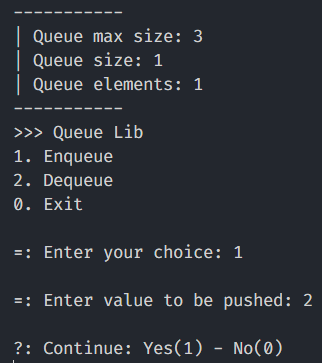
\includegraphics[width=\textwidth]{imgs/QueueArray/push/normal.png}
		\caption{Normal test cases}\label{fig:queue_arr_push_normal}
	\end{subfigure}
	\hfill
	\begin{subfigure}{0.59\textwidth}
		\centering
		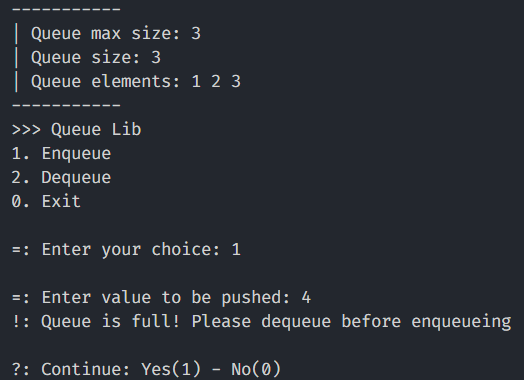
\includegraphics[width=\textwidth]{imgs/QueueArray/push/full.png}
		\caption{When the queue is full}\label{fig:queue_arr_push_full}
	\end{subfigure}
	\hfill
	\begin{subfigure}{0.75\textwidth}
		\centering
		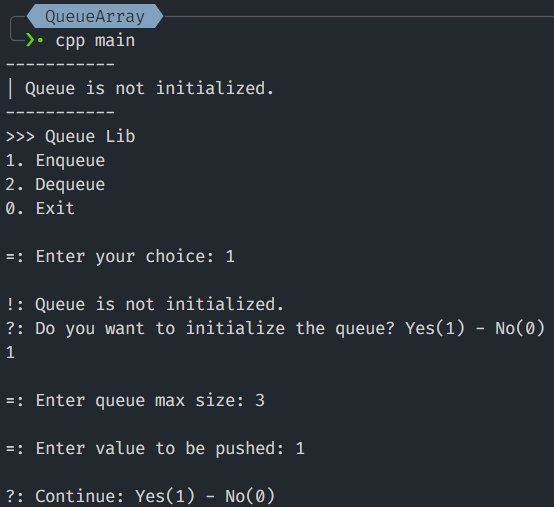
\includegraphics[width=\textwidth]{imgs/QueueArray/push/empty.png}
		\caption{When the queue is uninitialized}\label{fig:queue_arr_push_empty}
	\end{subfigure}
	\caption{Screenshots of queue (Array version) `push' operation.}\label{fig:queue_arr_push_cases}
\end{figure}
\subsubsection*{`dequeue' operation}
\begin{figure}[!ht]
	\centering
	\begin{subfigure}{0.6\textwidth}
		\centering
		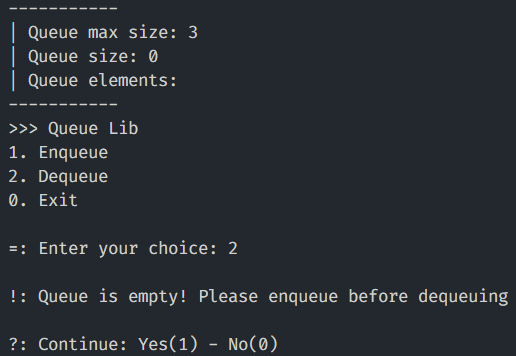
\includegraphics[width=\textwidth]{imgs/QueueArray/pop/empty.png}
		\caption{When the queue is empty}\label{fig:queue_arr_pop_empty}
	\end{subfigure}
	\hfill
	\begin{subfigure}{0.34\textwidth}
		\centering
		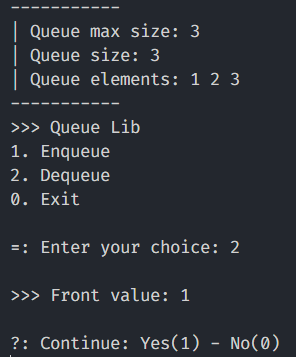
\includegraphics[width=\textwidth]{imgs/QueueArray/pop/normal.png}
		\caption{Normal test cases}\label{fig:queue_arr_pop_normal}
	\end{subfigure}
	\caption{Screenshots of queue (Array version) `pop' operation.}\label{fig:queue_arr_pop_cases}
\end{figure}

\pagebreak
\subsection{Queue (Linked List version)}
\subsubsection*{`enqueue' operation}
\begin{figure}[!ht]
	\centering
	\begin{subfigure}{0.55\textwidth}
		\centering
		\includegraphics[width=\textwidth]{imgs/queueLinkedList/push/empty.png}
		\caption{When the queue is uninitialized}\label{fig:queue_ll_push_empty}
	\end{subfigure}
	\hfill
	\begin{subfigure}{0.43\textwidth}
		\centering
		\includegraphics[width=\textwidth]{imgs/queueLinkedList/push/normal.png}
		\caption{Normal test cases}\label{fig:queue_ll_push_normal}
	\end{subfigure}
	\caption{Screenshots of queue (Linked List version) `push' operation.}\label{fig:queue_ll_push_cases}
\end{figure}
\subsubsection*{`dequeue' operation}
\begin{figure}[!ht]
	\centering
	\begin{subfigure}{0.6\textwidth}
		\centering
		\includegraphics[width=\textwidth]{imgs/queueLinkedList/pop/empty.png}
		\caption{When the queue is empty}\label{fig:queue_ll_pop_empty}
	\end{subfigure}
	\hfill
	\begin{subfigure}{0.34\textwidth}
		\centering
		\includegraphics[width=\textwidth]{imgs/queueLinkedList/pop/normal.png}
		\caption{Normal test cases}\label{fig:queue_ll_pop_normal}
	\end{subfigure}
	\caption{Screenshots of queue (Linked List version) `pop' operation.}\label{fig:queue_ll_pop_cases}
\end{figure}

\pagebreak
\section{Recursive versions}
\thispagestyle{empty}
\subsection{Stack}
\subsubsection*{Recursion Stack (Array version)}
\begin{itemize}
	\item \textbf{Theoretical Time Complexity:} Both implementations have the same theoretical time complexity of O(1) for \verb|push| and O(n) for \verb|copy| operations.
	\item \textbf{Practical Performance:}
	      \begin{itemize}
		      \item  Loop-based implementations are generally faster in practice because they avoid the overhead of function calls and recursion.
		      \item The recursive version doesn't work well with large data sets because of stack overflow.
	      \end{itemize}
\end{itemize}
\begin{figure}[!ht]
	\centering
	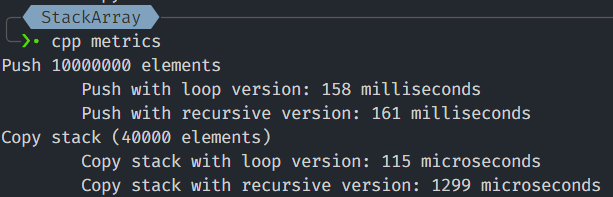
\includegraphics[width=0.6\textwidth]{imgs/StackArray/metrics.png}
	\caption{Recursive and loop version comparison of Stack (Array version)}\label{fig:stack_arr_metrics}
\end{figure}

\subsubsection*{Recursion Stack (Linked List version)}
\begin{itemize}
	\item \textbf{Theoretical Time Complexity:} Both implementations have the same theoretical time complexity of O(1) for \verb|push|, O(n) for \verb|copy| and \verb|release| operations.
	\item \textbf{Practical Performance:}
	      \begin{itemize}
		      \item  Loop-based implementations are generally faster in practice because they avoid the overhead of function calls and recursion.
		      \item The recursive version doesn't work well with large data sets because of stack overflow.
	      \end{itemize}
\end{itemize}
\begin{figure}[!ht]
	\centering
	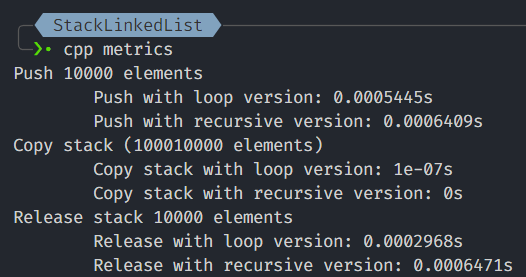
\includegraphics[width=0.6\textwidth]{imgs/StackLinkedList/metrics.png}
	\caption{Recursive and loop version comparison of Stack (Linked List version)}\label{fig:stack_ll_metrics}
\end{figure}
\thispagestyle{empty}
\subsection{Queue}
\subsubsection*{Recursion Queue (Array version)}
\begin{itemize}
	\item \textbf{Theoretical Time Complexity:} Both implementations have the same theoretical time complexity of O(1) for \verb|enqueue| and O(n) for \verb|copy| operations.
	\item \textbf{Practical Performance:}
	      \begin{itemize}
		      \item  Loop-based implementations are generally faster in practice because they avoid the overhead of function calls and recursion.
		      \item The recursive version doesn't work well with large data sets because of stack overflow.
	      \end{itemize}
\end{itemize}
\begin{figure}[!ht]
	\centering
	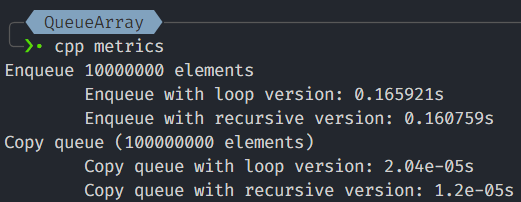
\includegraphics[width=0.6\textwidth]{imgs/QueueArray/metrics.png}
	\caption{Recursive and loop version comparison of Queue (Array version)}\label{fig:queue_arr_metrics}
\end{figure}

\subsubsection*{Recursion Queue (Linked List version)}
\begin{itemize}
	\item \textbf{Theoretical Time Complexity:} Both implementations have the same theoretical time complexity of O(1) for \verb|enqueue| and O(n) for  \verb|release| operations.
	\item \textbf{Practical Performance:}
	      \begin{itemize}
		      \item  Loop-based implementations are generally faster in practice because they avoid the overhead of function calls and recursion.
		      \item The recursive version doesn't work well with large data sets because of stack overflow.
	      \end{itemize}
\end{itemize}
\begin{figure}[!ht]
	\centering
	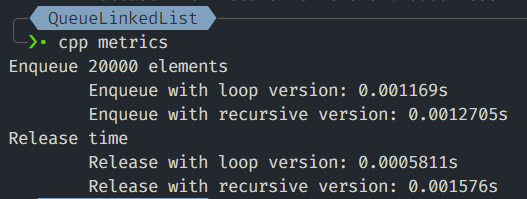
\includegraphics[width=0.6\textwidth]{imgs/QueueLinkedList/metrics.png}
	\caption{Recursive and loop version comparison of Queue (Linked List version)}\label{fig:queue_ll_metrics}
\end{figure}

\pagebreak
\section{Self-evaluation}
\begin{center}
  \renewcommand{\arraystretch}{1.5}
  \begin{tabular}{|l|p{\dimexpr0.6\linewidth-2\tabcolsep}|c|}
    \hline
    \textbf{No.} & \textbf{Details}            & \textbf{Score} \\ \hline
    1            & Stack (Array version)       & 100\%          \\ \hline
    2            & Stack (Linked List version) & 100\%          \\ \hline
    3            & Queue (Array version)       & 100\%          \\ \hline
    4            & Queue (Linked List version) & 100\%          \\ \hline
    5            & Recursive versions          & 100\%          \\ \hline
    6            & Report                      & 100\%          \\ \hline
  \end{tabular}
\end{center}

\section{Exercise Feedback}
\subsection{What I learned}
\begin{flushleft}
  Because almost the things could be done easily, I have learned nothing new from this exercise.
\end{flushleft}
\subsection{What I found challenging}
\begin{flushleft}
  This exercise is quite simple and easy, so I have no difficulties to finish this task.
\end{flushleft}
\subsection{What I have used in this exercise}
\begin{itemize}
  \item I used C++ to implement the data structures and the test cases.
  \item I also used \LaTeX{} to write this report.
  \item All the source code and the report are available in \href{https://github.com/yuran1811/}{my github repo}
\end{itemize}
\end{document}